\documentclass[11pt, letterpaper]{article}
\usepackage[utf8]{inputenc}
\usepackage[letterpaper, margin=0.5in]{geometry}
\usepackage{amsmath}
\usepackage{amssymb}
\usepackage{amsthm}
\usepackage{graphicx}
\usepackage{listings}
\usepackage[font=scriptsize]{caption}
\usepackage{subcaption}
\usepackage{xcolor}

\definecolor{codegreen}{rgb}{0,0.6,0}
\definecolor{codegray}{rgb}{0.5,0.5,0.5}
\definecolor{codepurple}{rgb}{0.58,0,0.82}
\definecolor{backcolour}{rgb}{0.95,0.95,0.92}

\lstdefinestyle{mystyle}{
    backgroundcolor=\color{backcolour},   
    commentstyle=\color{codegreen},
    keywordstyle=\color{magenta},
    numberstyle=\tiny\color{codegray},
    stringstyle=\color{codepurple},
    basicstyle=\ttfamily\footnotesize,
    breakatwhitespace=false,
    texcl=true,
    mathescape=true,
    breaklines=true,                 
    captionpos=b,                    
    keepspaces=true,                 
    numbers=left,                    
    numbersep=5pt,                  
    showspaces=false,                
    showstringspaces=false,
    showtabs=false,                  
    tabsize=2
}

\lstset{style=mystyle}
\graphicspath{ {.} }
\captionsetup{justification=raggedright, singlelinecheck=false}

\author{Ryan Tang}
\title{STA 602 HW 10}
\date{November 11th 2022}

\begin{document}
\maketitle

\section{Exercise 7.4}
\paragraph{(a)}
Here I decided to use a prior that doesn't contain much information with a sprinkle of my guesses.
\begin{align*}
    Y_i &\mathop{\thicksim}^{iid} \mathcal{N}(\theta, \Sigma) \\
    \theta &\thicksim \mathcal{N}(\theta|
        \mu_0=\begin{bmatrix}35\\33\end{bmatrix},
        \Sigma_0=\begin{bmatrix}5,0\\0,5\end{bmatrix}
    ) \\
    \Sigma &\thicksim IW(\Sigma|\nu_o = 3, S_o =\begin{bmatrix}100,60\\60,100\end{bmatrix})
\end{align*}

\paragraph{(b)}
Below are 3 draws of prior predictive distribution samples resulting from the above prior specifications.
\begin{figure*}[!h]
  \centering
  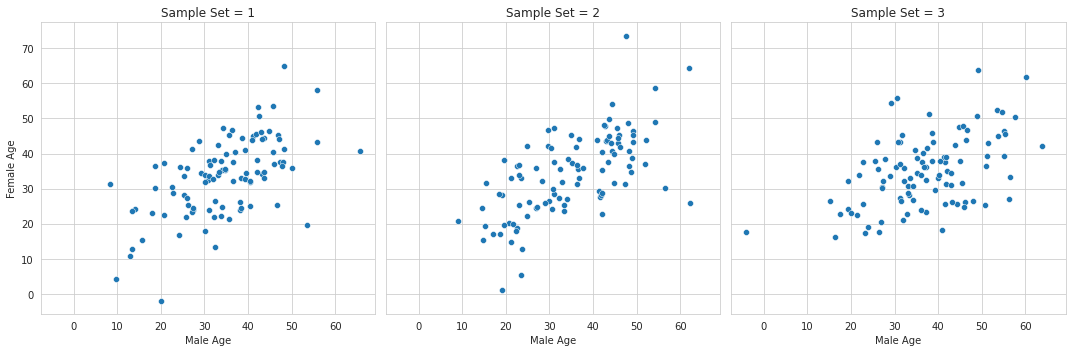
\includegraphics[width=1.0\textwidth]{1.a.png}
  \captionsetup{justification=centering}
  \caption{Prior Predictive of $Y$}
\end{figure*}

\paragraph{(c)}
Now, we draws posterior samples from the full conditionals using a Gibbs Sampler with the provided dataset $Y$.
\begin{align*}
    \theta|Y, \Sigma &\thicksim \mathcal{N}(\theta|\mu_n, \Sigma_n) \\
    \Sigma_n &= (\Sigma_0^{-1} + N \Sigma^{-1})^{-1} \\
    \mu_n &= \Sigma_n (\Sigma^{-1}N\bar{Y} + \Sigma_0^{-1}\mu_o) \\ \\
    \Sigma|Y &\thicksim IW(\nu_o, S_n) \\
    \nu_n &= \nu_o + N \\
    S_n &= S_o + S_\theta \\
    S_\theta &= \sum_i^N (y_i - \theta)(y_i - \theta)^{\intercal}
\end{align*}

Below are the plots for the joint $\theta$ posterior and the marginal posterior correlation distribution between $Y_h$ and $Y_w$.
We also obtained statistics around $\theta|Y$, too. $\theta_h|Y$ and $\theta_w|Y$ has around 0.903 correlation. $\theta_h|Y$'s
95\% confidence interval lies between $[43.35, 46.90]$, and $\theta_w|Y$'s 95\% confidence interval lies between $[39.88, 43.18]$.
\begin{figure*}[!h]
  \centering
  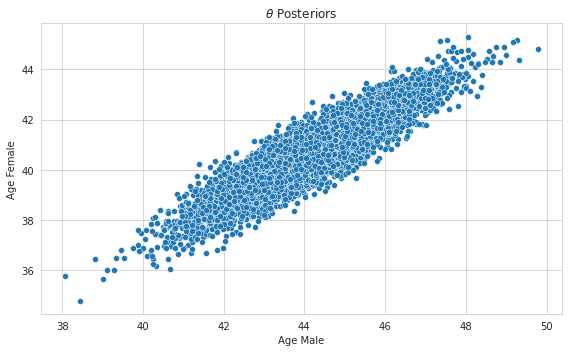
\includegraphics[width=0.5\textwidth]{1.b.png}
  \captionsetup{justification=centering}
  \caption{$\theta$ Posterior Joint}
\end{figure*}
\begin{figure*}[!h]
  \centering
  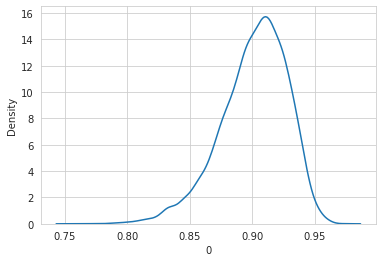
\includegraphics[width=0.5\textwidth]{1.c.png}
  \captionsetup{justification=centering}
  \caption{$Y$ correlation distribution}
\end{figure*}

\paragraph{(d.i) Jeffery Priors}
Using Jeffery Priors, we can see the chain is slow on convergence.
\begin{itemize}
    \item $\mu_o=0, \Sigma_o=\mathbf{I}, \nu_o=1, S_o = \mathbf{0}$
    \item Posterior correlation $0.213$
    \item $\theta_h|Y$'s 95\% confidence interval lies between $[0.64, 2.99]$
    \item $\theta_w|Y$'s 95\% confidence interval lies between $[0.35, 2.72]$
\end{itemize}

\paragraph{(d.ii) Unit Information Priors}
Using Unit Information Priors with MLE:
\begin{itemize}
    \item Posterior correlation $0.907$
    \item $\theta_h|Y$'s 95\% confidence interval lies between $[43.46, 47.11]$
    \item $\theta_w|Y$'s 95\% confidence interval lies between $[39.98, 43.44]$
\end{itemize}

\paragraph{(d.iii) Diffuse Priors}
Using an extremely diffuse prior pair:
\begin{itemize}
    \item Posterior correlation $0.853$
    \item $\theta_h|Y$'s 95\% confidence interval lies between $[43.47, 47.17]$
    \item $\theta_w|Y$'s 95\% confidence interval lies between $[40.00, 43.48]$
\end{itemize}

\paragraph{(e)}
I certainly think my priors helped quite a lot, especially compared to the Jeffery priors. Although Jeffery priors don't contain any information, assuming the means are zeros made the Gibbs sampler slower. Unit Information Priors tend to over-fit because
it relies on observation data and MLE estimates. Diffuse priors can slow down the learning process if we have good domain knowledge of the subject, like in our case here.

Hypothetically speaking, we end up with 25 samples instead of 100; diffuse priors will perform worse because it wants more data. And Unit Information priors will end up over-fitting easily because of the high MLE estimation variances with small data size. Jeffery priors can work; we need a better sampler than the Gibbs we are using now. However, if we are concerned about the code start issue, we should inject some knowledge into the prior instead of relying on a pair of uninformative priors.


\newpage
\section{Exercise 7.5}
\paragraph{(a) Some Statistics on Observed Data}
Due to missing data, here we only calculated the statistics on the observed portion of the data.
\begin{itemize}
    \item Mean: $\hat{\theta}_{A_{obs}} = 24.20, \hat{\theta}_{B_{obs}} = 24.81$
    \item Variances: $\hat{\sigma}^2_{A_{obs}} = 4.09, \hat{\sigma}^2_{B_{obs}} = 4.69$
    \item Correlation: $\hat{\rho}_{obs} = 0.616$
\end{itemize}

\paragraph{(b)}
We imputed the data using missing at random assumption and multivariate normal sampling model. After we arrived at the imputed dataset, we ran a t-test on $\theta_A - \theta_B$ to see if there were any significant differences between the two response times. The t-test came back with some good results saying that we rejected the null hypothesis. See Figures (4) and (5) for details.
\begin{itemize}
    \item t-statistics $= -3.455$, p-value $= 0.0018$
    \item 95\% Confidence Interval $[-3.45, 2.332]$
\end{itemize}

\begin{figure*}[!h]
  \centering
  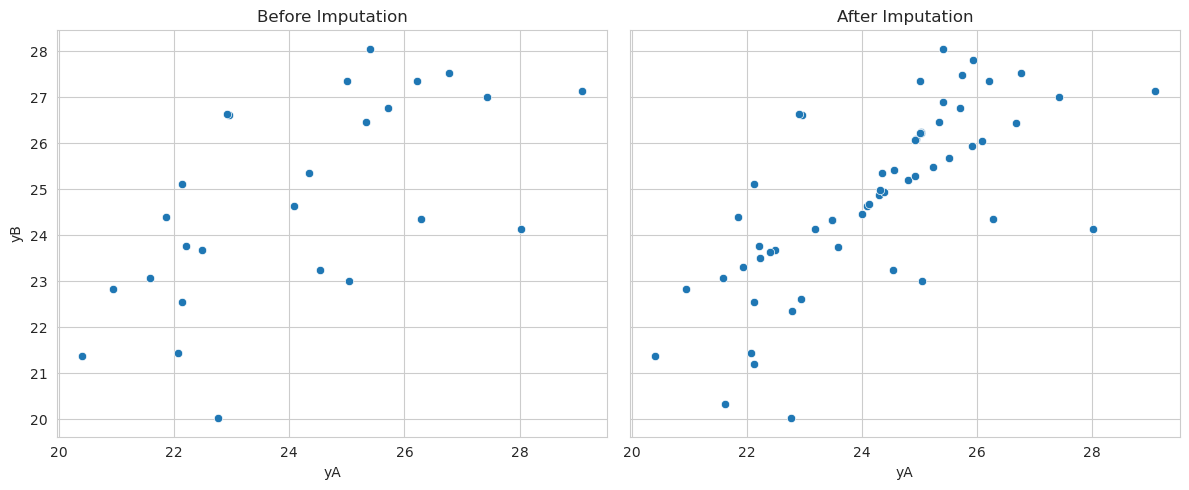
\includegraphics[width=0.85\textwidth]{2.a.png}
  \captionsetup{justification=centering}
  \caption{Imputation before and after comparison}
\end{figure*}
\begin{figure*}[!h]
  \centering
  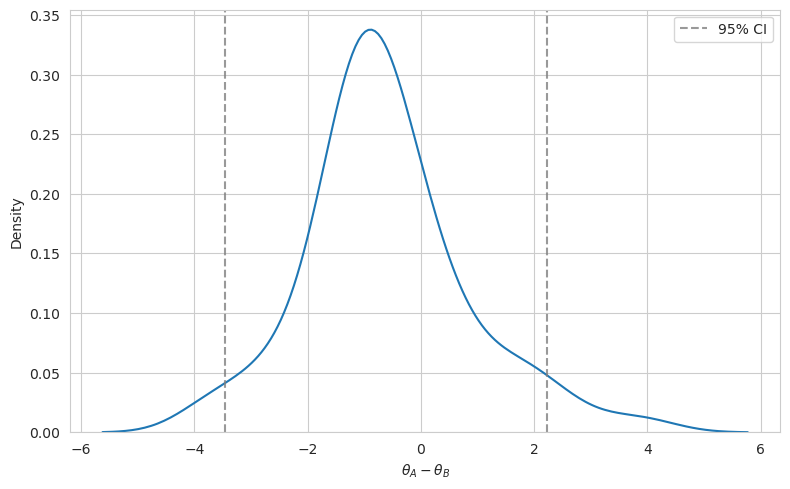
\includegraphics[width=0.6\textwidth]{2.b.png}
  \captionsetup{justification=centering}
  \caption{$\theta_A$ - $\theta_B$ Density}
\end{figure*}

\paragraph{(c) Gibbs Sample with MVN Imputation}
Lastly, we use the Gibbs sampler to do the imputation and calculate the statistics about $\theta_A - \theta_B$. The posterior density is shown below in Figure 6.
\begin{itemize}
    \item The posterior mean is -0.615 
    \item 95\% Confidence Interval $[-1.016, -0.207]$
\end{itemize}
\begin{figure*}[!h]
  \centering
  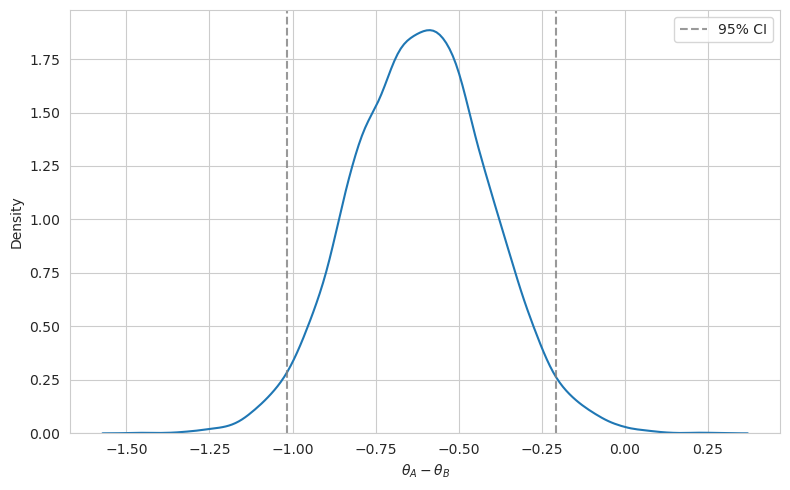
\includegraphics[width=0.6\textwidth]{2.c.png}
  \captionsetup{justification=centering}
  \caption{$\theta_A$ - $\theta_B$ Density - Gibbs Sampler}
\end{figure*}

\paragraph{Appendix}
The code for generating the posterior samples is included here for completeness.
\begin{lstlisting}[language=Python]
import pandas as pd
import numpy as np
import scipy.stats as stats
from numpy.linalg import inv
from numpy.random import multivariate_normal
from scipy.stats import invwishart

class MVNMean:
    def __init__(self, $\mu$0, $\Sigma$0):
        self.$\mu$0 = $\mu$0
        self.$\Sigma$0 = $\Sigma$0
        self.$\Lambda$0 = inv($\Sigma$0)
    
    def sample_prior(self, size=1):
        return multivariate_normal(self.$\mu$0, self.$\Sigma$0, size=size)
    
    def sample_posterior(self, X, $\Sigma$, size=1):
        n = X.shape[0]
        X_mean = X.mean(axis=0)

        $\Lambda$ = inv($\Sigma$)
        $\Lambda$n = self.$\Lambda$0 + n * $\Lambda$
        $\Sigma$n = inv($\Lambda$n)
        $\mu$n = $\Sigma$n @ ($\Lambda$ @ (n*X_mean) + self.$\Lambda$0 @ self.$\mu$0)
        return multivariate_normal($\mu$n, $\Sigma$n, size=size)

class MVNSigma:
    def __init__(self, v0, S0):
        self.v0 = v0
        self.S0 = S0
    
    def sample_prior(self, size=1):
        return invwishart(self.v0, self.S0).rvs(size=size)
    
    def sample_posterior(self, X, $\theta$, size=1):
        n = X.shape[0]
        S = (X - $\theta$).T @ (X - $\theta$)

        vn = self.v0 + n
        Sn = self.S0 + S
        return invwishart(vn, Sn).rvs(size=size)

def impute_B(B_mean, yA, A_mean, B_var, A_var, rho):
    return B_mean + (yA - A_mean) * np.sqrt(B_var/A_var) * rho

def impute_A(A_mean, yB, B_mean, A_var, B_var, rho):
    return A_mean + (yB - B_mean) * np.sqrt(A_var/B_var) * rho

def cov2corr($\Sigma$):
    var = np.diag($\Sigma$).reshape(-1, 1)
    return $\Sigma$ / np.sqrt(var @ var.T)

def impute_X(X, $\theta$, $\Sigma$):
    $\theta$A, $\theta$B = $\theta$
    $\sigma$2A, $\sigma$2B = $\Sigma$[0,0], $\Sigma$[1,1]
    $\rho$ = cov2corr($\Sigma$)[0,1]

    imputed_X = []
    for (yA, yB) in X:
        if np.isnan(yA):
            imputed_X.append((impute_A($\theta$A, yB, $\theta$B, $\sigma$2A, $\sigma$2B, $\rho$), yB))
        elif np.isnan(yB):
            imputed_X.append((yA, impute_B($\theta$B, yA, $\theta$A, $\sigma$2B, $\sigma$2A, $\rho$)))
        else:
            imputed_X.append((yA, yB))

    return np.array(imputed_X)

# get data
df = pd.read_fwf("interexp.dat")
X = df.values
N = df.shape[0]

# prior parameters
$\theta$_rv = MVNMean(
    $\mu$0 = df.mean().values,
    $\Sigma$0 = df.dropna().cov().values
)

$\Sigma$_rv = MVNSigma(
    v0 = 2,
    S0 = df.dropna().cov().values
)

samples = []
nEpochs = 10000
$\Sigma$ = $\Sigma$_rv.sample_prior()
$\theta$ = $\theta$_rv.sample_prior().ravel()
imputed_X = impute_X(X, $\theta$, $\Sigma$)
for epoch in range(nEpochs):
    $\theta$ = $\theta$_rv.sample_posterior(imputed_X, $\Sigma$).ravel()
    $\Sigma$ = $\Sigma$_rv.sample_posterior(imputed_X, $\theta$)
    imputed_X = impute_X(X, $\theta$, $\Sigma$)

    diff = $\theta$[0] - $\theta$[1]

    samples.append(($\theta$, $\Sigma$, diff))
\end{lstlisting}



\newpage
\section{Exercise 7.6}
\paragraph{(a) Separate Posterior Parameters Comparisons}
Below graph shows the comparison between $\theta_{d, j}$ and $\theta_{n, j}$. At the same time, we also calculated the $P[\theta_{d, j} > \theta_{n, j}|Y]$. The obtained probability was all 100\% $\forall j \in \{1\dots7\}$.
\begin{figure*}[!h]
  \centering
  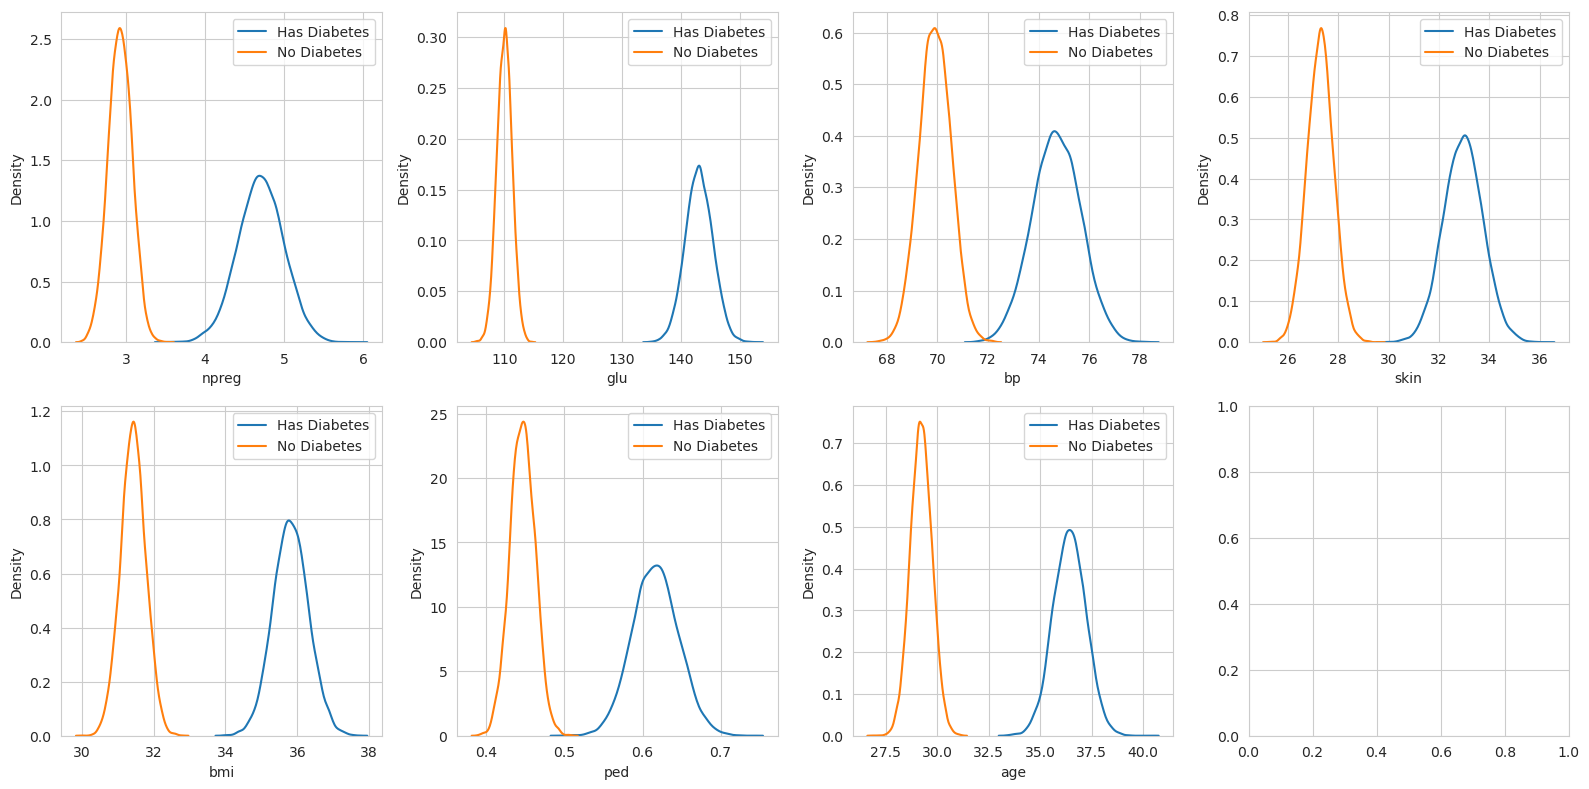
\includegraphics[width=1.0\textwidth]{3.a.png}
  \captionsetup{justification=centering}
  \caption{Posterior Comparison between the two groups}
\end{figure*}

\paragraph{(b) $\Sigma|Y$ Comparison}
Lastly, we investigate the covariance samples. I averaged over all sampled posterior covariance for each group and plotted each entry color coded by the group. Below is the graph.
\begin{figure*}[!h]
  \centering
  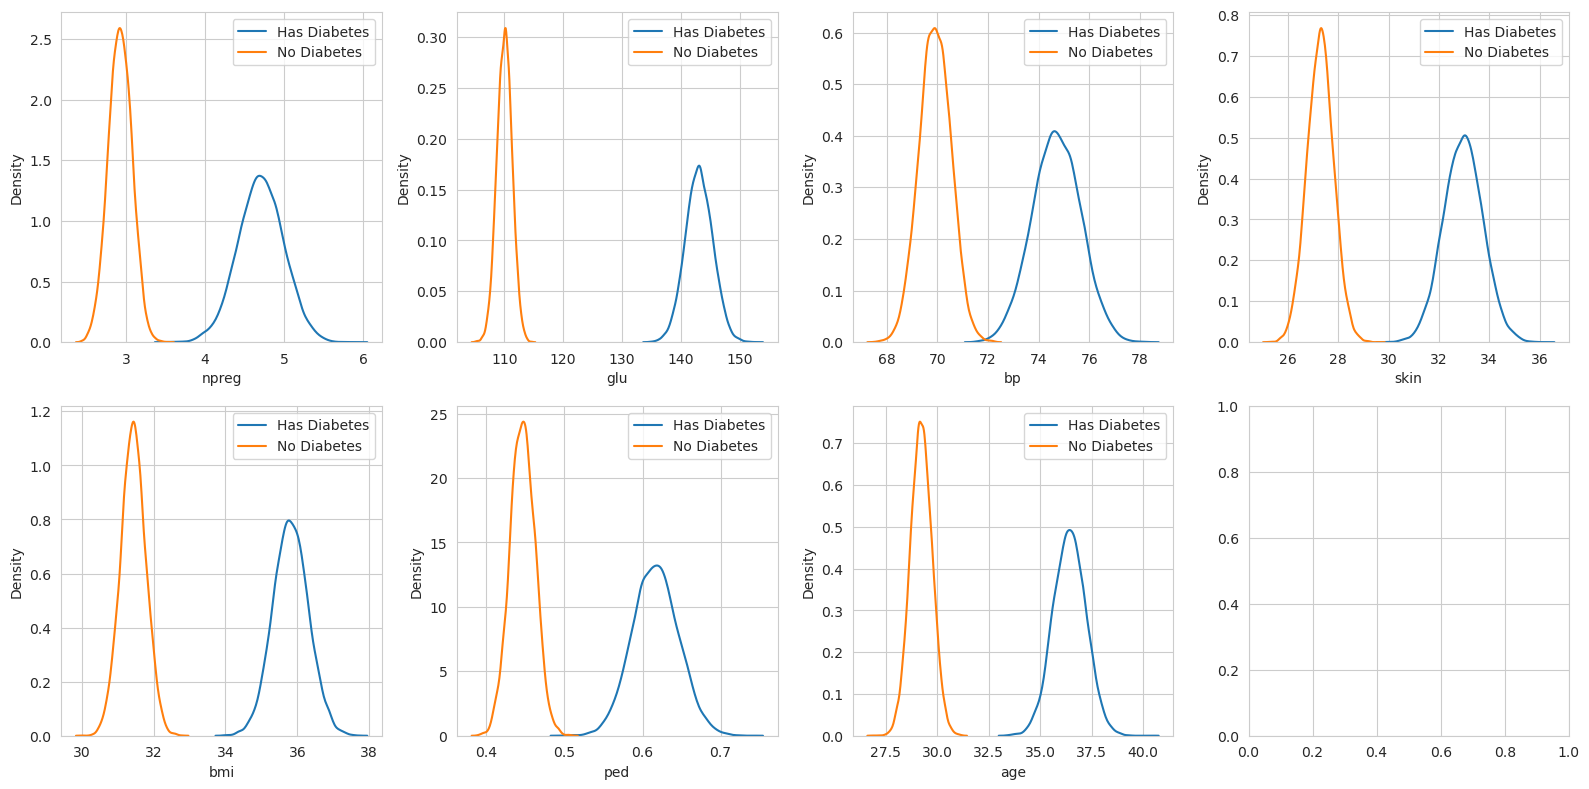
\includegraphics[width=1.0\textwidth]{3.a.png}
  \captionsetup{justification=centering}
  \caption{Posterior Comparison between the two groups}
\end{figure*}

\end{document}